\chapter{Instrukcja użytkownika}

\section{Wersja Pordukcyjna}
Wersja produkcyjna aplikacji jest uruchomiona na serwerze heroku, pod adresem \url{http://terrain-editor.herokuapp.com}{http://terrain-editor.herokuapp.com}

Pierwsze uruchomienie wymaga uruchomienia serwera, który przechodzi w stan uśpienia po godzinie braku aktywności ze strony użytkowników w celu oszczędności zasobów. Z tego powodu po wpisaniu adresu w przeglądarce internetowej po raz pierwszy, należy zaczekać nieco dłużej niż w przypadku kolejnych zapytań do serwera.

\subsection{Logowanie i rejestracja}
Aby mieć dostęp do wszystkich funkcji aplikacji, należy się zalogować, lub zarejestrować nowego użytkownika.

Ze względu na przeznaczenie projektu do celów edukacyjnych, postanowiłem nie walidować adresów email pod kątem prawdziwości, dlatego dopuszczalne do rejestracji są fałszywe adresy, pod warunkiem że zachowany zostanie poprawny format.

W wersji pokazowej zarejestrowany został użytkownik:
\textbf{email:} test.user@example.com
\textbf{hasło:} password

\FloatBarrier
 	\begin{figure}[ht]
        \centering
        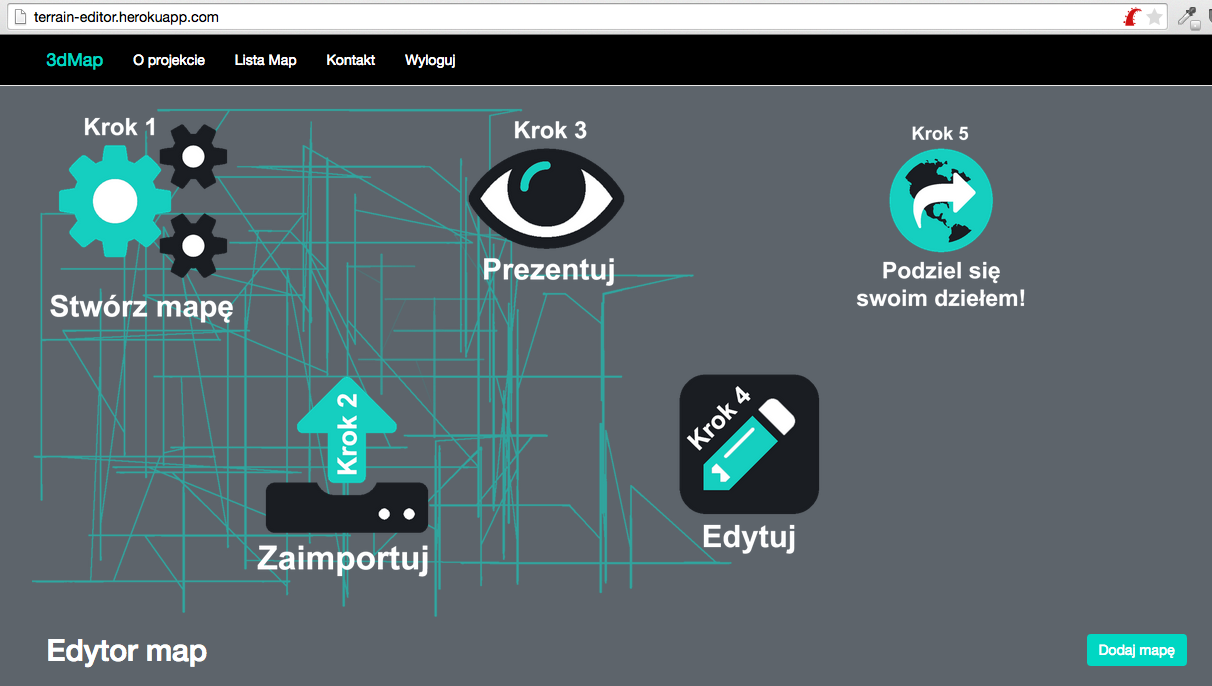
\includegraphics[width=0.90\textwidth,height=0.46\textheight]{img/home.png}
	\caption{Strona główna aplikacji}
        \label{rys:screen_home}
    \end{figure}
\FloatBarrier
	
\subsection{Kontrola dostępu}

Wykorzystanie sesji logowania pozwoliło na ograniczenie praw dla użytkowników niezalogowanych, jak i dla zalogowanych.

\begin{itemize}
\item Użytkownicy niezalogowani mogą:
	\subitem Przeglądać mapy
	\subitem Logować się, i rejestrować
	\subitem Wysyłać emaile kontaktowe
			
\item Użytkownicy zalogowani mogą:
	\subitem Wykonywać wszystkie akcje niezalogowanych użytkowników z wyjątkiem rejestracji i logowania.
	\subitem Dodawać mapy
	\subitem Edytować swoje mapy
\end{itemize}

W przypadku próby wykonania akcji zabronionej, użytkownik niezalogowany jest przekierowywany do ekranu logowania, zaś zalogowany użytkownik do strony głównej.

Na górze ekranu pojawi się wiadomość o braku uprawnień do wykonania danej akcji.

\FloatBarrier
 	\begin{figure}[ht]
        \centering
        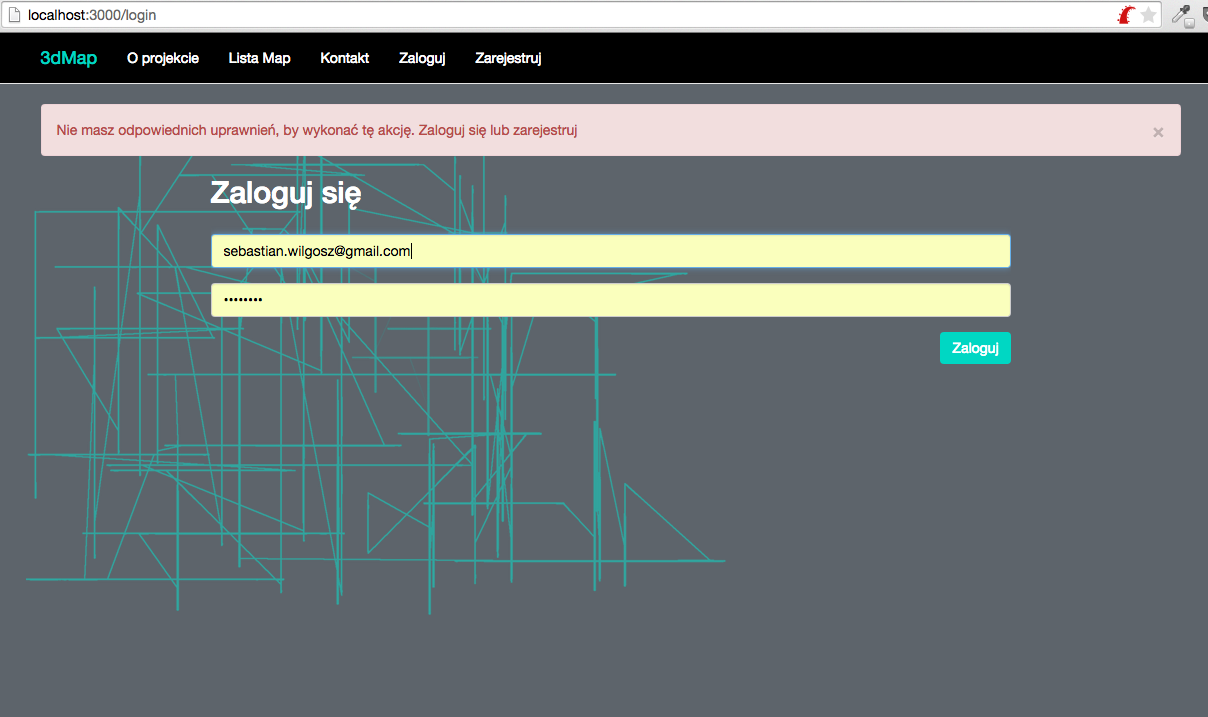
\includegraphics[width=0.90\textwidth,height=0.46\textheight]{img/no_access.png}
	\caption{Próba wykonania akcji zabronionej}
        \label{rys:screen_no_access}
    \end{figure}
\FloatBarrier

\subsection{Wysyłanie emaili}

Aplikacja umożliwia wysłanie wiadomości kontaktowej do administratorów systemu. Z powodu udostępnienia aplikacji online, postanowiłem wyłączyć funkcję wysyłania maili na rzeczywistą skrzynkę odbiorczą. Zamiast tego zintegrowałem projekt z aplikacją \textit{Mailtrap}, która przechwytuje wszystkie emaile wysyłane z konta pocztowego. W celu rekonfiguracji konta, zobacz sekcję: \ref{dev_mailer}.

\subsection{Dodawanie mapy z pliku}

Dodawanie nowych map jest dostępne wyłącznie dla zalogowanych użytkowników. Jeżeli chcesz dodać mapę, będąc zalogowanym kliknij w przycisk na stronie głównej, liście map albo stornie pojedynczej mapy.

\FloatBarrier
 	\begin{figure}[ht]
        \centering
        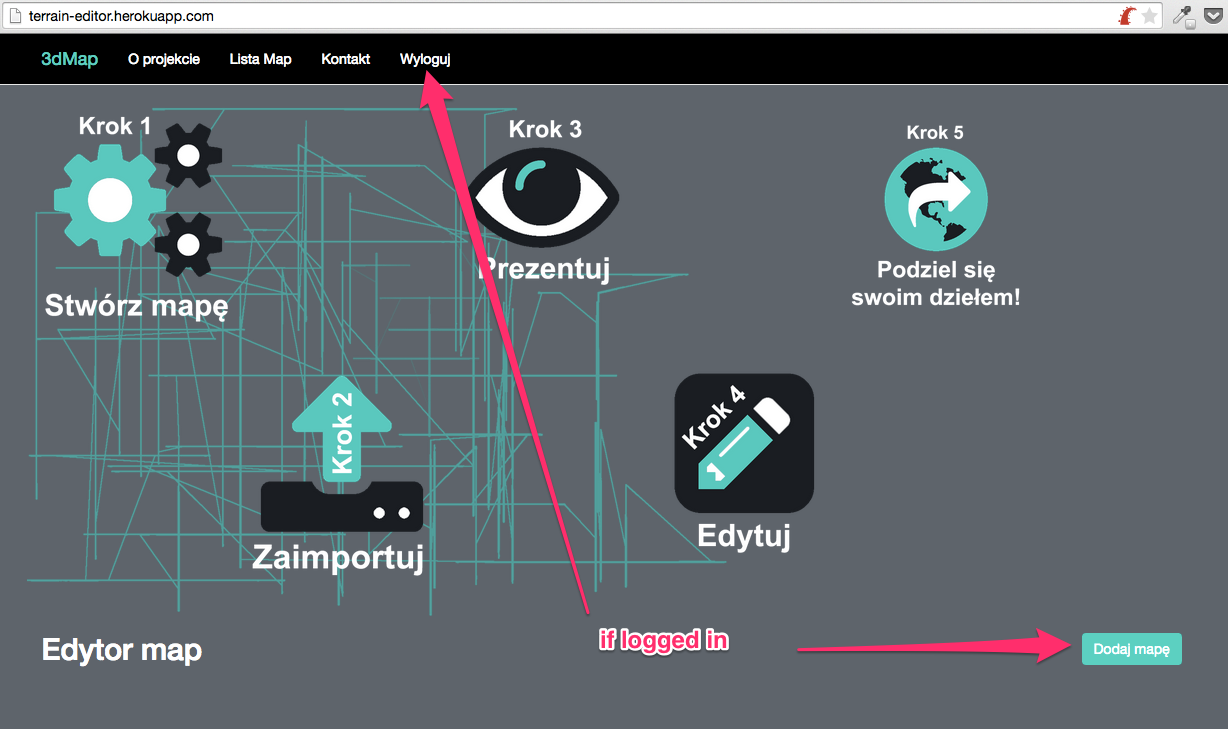
\includegraphics[width=0.90\textwidth,height=0.46\textheight]{img/add_map1.png}
	\caption{Dodawanie mapy, krok 1}
        \label{rys:screen_add_map1}
    \end{figure}
\FloatBarrier

Po kliknięciu w przycisk pojawi się formularz dodawania nowej mapy. Schemat należy wczytać z odpowiednio sformatowanego pliku tekstowego.

Plik powinien mieć następujący format:

\begin{table}[h]
	\centering
	\begin{tabular}{|l|l|l|l|l|l|}
		Source X & Source Y & Source Z & Target X & Target Y & Target Z \\ \hline
	\end{tabular}
	\caption{Format pliku z danymi mapy do importu.}
	\label{tab:file_format}
\end{table}

Lub powinine być plikiem tekstowym, w którym każda linia odpowiada kolejnemu wierszowi, zaś komórki są oddzielone średnikiem (";").

W celach prezentacyjnych do repozytorium zostały dołączone przykładowe pliki z danymi do zaimportowania w katalogu \textit{app/assets/csv/*}.

Jeżeli import mapy przebiegł poprawnie, użytkownik zostanie przekierowany do widoku właśnie dodanej mapy.

\FloatBarrier
 	\begin{figure}[ht]
        \centering
        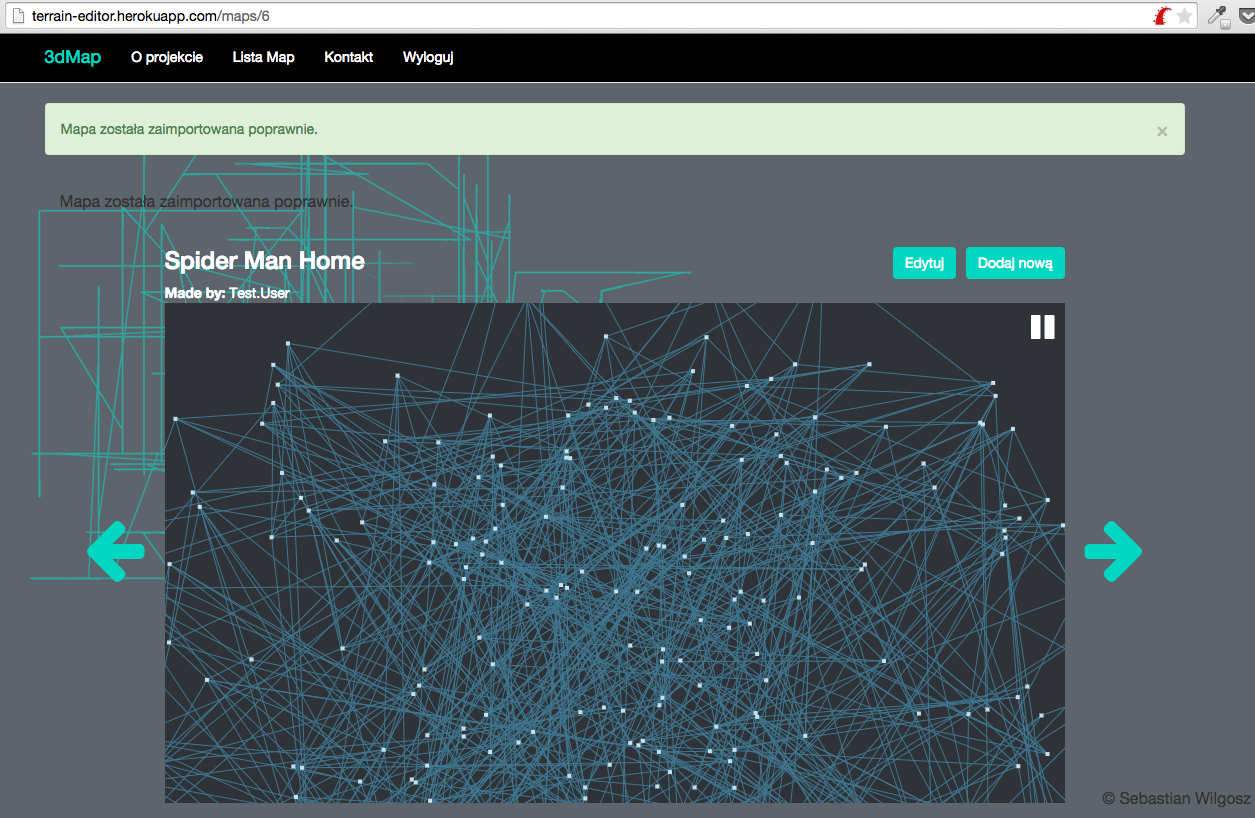
\includegraphics[width=0.90\textwidth,height=0.46\textheight]{img/add_map2.png}
	\caption{Widok mapy}
        \label{rys:screen_show_map}
    \end{figure}
\FloatBarrier

Ten ekran wyświetla mapę jako obracającą się wizualizację 3D. Użytkownik może zatrzymać i wznowić animację, klikając w iconę w prawym górnym rogu animacji.

Ponadto użytkownik może w prosty sposób przeglądać inne mapy zapisane na serwerze, klikając w strzałki po prawej i lewej stronie.

\section{Wersja lokalna}

ubuntu/reverse

\subsection{Wysyłanie emaili}
\label{dev_mailer}